\documentclass{report}

\usepackage{amsmath}
\usepackage{graphicx}
\usepackage{hyperref}
\usepackage{cleveref}

\graphicspath{ {./figures/} }

\begin{document}

\title{Scale- and Translation-Invariant Unsupervised Learning of Hidden Causes Using Spiking Neurons with Selective Visual Attention}
\author{Youssef Kashef\\
\\
\\
Submitted in Partial Fulfillment of the Requirements\\
for the Degree of Master-Diplom\\
in Neural Systems and Computation\\
at\\
ETH Z{\"u}rich\\
\\
}
\date{7. August 2013}

\maketitle
\tableofcontents

\begin{abstract}

Nessler et al. have demonstrated the ability of a spiking neuronal network governed by spike-timing-dependent-plasticity (STDP) and a stochastic winner-take-all (WTA) circuit to learn and predict causes from visual input. We aim to increase the computational power of the existing network through invariance to translation and scale. The visual system of the brain masters the recognition of objects wherever they appear in the visual scene, regardless of scale, orientation or even with partial occlusions. It leverages this through attention. Therefore, we turn to the pool of literature on modeling visual attention systems inspired from the brain. The architecture of the extended model is composed of the existing recognition module receiving bottom-up input from an attention module. Pre-attentive computations allow the attention module to alter the input window exposed for recognition. Attention is modeled as a network measuring for saliency in a scene by feature extraction with the use of hierarchies. The design and development of this extended model to achieve the required invariance by using processes that approximate their biological counterparts is presented. Emphasis is put on making these approximations through computationally economic implementations. Evaluation of the model is based on its performance and convergence in a set of experiments as well as its computational efficiency. Experiments are constructed to scrutinize the behavior of the model, its ability to converge onto a sight within a scene that enables recognition. Artificial data as well as images of handwritten digits are used to further reveal the capabilities and limitations of our approach. A top-down feedback signal of the recognition module that modulates attention is discussed.

\end{abstract}

\chapter{Introduction}

\paragraph{}\textbf{Spike-based Expectation Maximization (SEM)} is a model of Bayesian modules articulated by Nessler et. al of how the brain analyzes sensory stimuli. The model demonstrates the learning of hidden causes in visual stimuli emerging through correlations in a stochastic soft winner-take-all (WTA) network of spiking neurons. The spiking neurons are activated continuously in the presence of their preferred stimulus \cite{Nessler2010}. Spike-timing-dependent-plasticity (STDP) in WTA circuits defines the learning method for recognizing the hidden causes in the stimulus. The utilization of STDP acts as an approximation of traditional Expectation Maximization \cite{Nessler2013}. This model forms the basis of the presented work.

More emphasis will be put on how the WTA circuit in the SEM model is constructed and utilized. This WTA circuit constitutes our main building block. It comprises of a feed-forward single layer spiking neural network. The input layer is made out of spiking nodes whose firing activity is governed  by a Poisson process. External variables undergo a population coding that determines the modality of this Poisson process. In the example offered by Nessler et al, the external variables are pixel intensity values, form a static visual image stimulus. The population coding polarizes the pixel intensity values into binary On-Off states which directly determine the firing probability of the Poisson process. A spiking neuron is assigned to encode each state of the population code generated for each pixel. In this case, two spiking nodes per pixel. An On-node and an Off-node. The firing rate of these neurons is proportional to the state of the node in the population code \cite{Nessler2010}.

\paragraph{}\textbf{Selective Attention} delivers a strategy to economize computational power and reduce its entropy. Its evolutionary motivation comes for the organism's need to detect prey rapidly. Itti et al. propose a framework for attention involving interactions between bottom-up cues that are stimulus driven and top-down cues that are task-dependent \cite{Itti2001}. The bottom-up cues are triggered by a mechanism for static feature detection and possibly also temporal event detection. Top-down attention may originate from predictive mechanisms that bias selectivity. Top-down cues may also arise from independent motor control \cite{Olshausen1993}. A third methodology for reaching invariance, yet not solely through attention is one demonstrated by Leibo et al, where they leverage temporal association in natural vision when viewing an object for creating invariant templates of this object \cite{Leibo2010}

Extending the SEM model with feature-based modules and providing input that is previously filtered by an attention module we provides a reduction in dimensionality increase in computational efficiency and invariance to scale and translation.

\chapter{Methods}
\section{Object Recognition using Spike-based Expectation Maximization}

\subsection{Extending SEM by learning orientations}

The original SEM model is made out of an input layer receiving signals from external variables $x$. Population codes determine the state of a set of spiking neurons $y$ for each node $x$. The spiking pattern of each node $y$ follows a Poisson process. Spikes generated from all $y$ neurons serve as input to a WTA circuit of $z$ neurons with weights $\textbf{w}$ for each neuron. The $z$ neurons form the output layer. The use of notations $x$, and $z$ is to draw the connection to the Expectation Maximization algorithm that the model approximates. As it tries to maximize $E_p*[log \hspace{5 pt} p(y|\textbf{w})]$ with $q(z|y)=p(z|y,\textbf{w}^{old})$ in the E-Step, where $\textbf{w}^{old}$ is the weight vector for each of the $z$ neurons and replacing $\textbf{w}$ with updated weights for the M-step \cite{Nessler2010, Nessler2013, Habenschuss2013}.
Applied to an example, $x$ variables are pixels from a static image of a handwritten digit. Two $y$ neurons fire antognistically, depending on the intensity level of their associated $X$ node (where $X\in x$). Neurons in the $z$ layer produce a firing pattern that is distinct for to the hidden cause. The handwritten digits can be categorized into distinct classes and we see that the SEM can produce a unique firing pattern for each class through unsupervised learning \cite{Nessler2010}. 

\paragraph{}We will keep the WTA circuit as our main building block. We will also preserve the hebbian learning rule \ref{eqn_rule} to update the weights of $z$ neurons to use for the M-Step \cite{Nessler2010}. The population coding for polarizing intensity values to drive the Poisson process will remain useful, but the population coding will also be the first entry point for the extensions.

\begin{equation}
	    \Delta w_{ki}= 
			\begin{cases}
			    \eta (1-\exp^{w_{ki}}), & \text{if } y_i=1 \text{ and } z_k=1\\
			    -\eta,                  & \text{if } y_i=0 \text{ and } z_k=1\\
			    -0                      & \text{if } z_k=0\\
			\end{cases}
	\label{eqn_rule}
\end{equation}
where $w_{ki}$ denotes the $i$th component of the weight vector $\textbf{w}_k$ for learner $k$.
and in the special case of the neuron's bias $i$=0:
\begin{equation}
	    \Delta w_{k0}= 
			\begin{cases}
			    \eta (1-\exp^{w_{k0}}), & \text{if } z_k=1\\
			    -\eta,                  & \text{if } z_k=0\\
			\end{cases}
	\label{eqn_rule_bias}
\end{equation}

The current encoding of external variables accounts for the intensities of the spatial units, pixels, of the presented stimulus. The encoding of intensities is performed through a population coding by antagonistic binary nodes per pixel that drive a Poisson process \cite{Nessler2010}. Parallel to these intensity-encoded nodes, we add a WTA circuit per pixel that determines the preferred orientation of this node relative to its spatial neighbors. This creates an orientation map of the presented stimulus. While counter-intuitive with traditional learning models, SEM benefits from elaborating the dimensionality of WTA's feature space as this increases its resolution for detecting correlations between an output node $z$ and input nodes $y$ on a linear scale. Since SEM aims to reduce dimensionality, it is preferable to describe it as an elaboration of dimensionality. The added dimensions, or nodes, do not carry new information, but rather refine its representation. Recalling the use of population coding to encode in atagonistic (On-node, Off-node) fashion, thus letting the WTA learn the likelihood of an input node firing and not firing explicitly, as shown by \ref{eqn_corr}.

\begin{equation}
	p(z=1|y) \propto y*p(y=1|z) + (1-y)*p(y=0|z)
	\label{eqn_corr}
\end{equation}

where
\begin{itemize}
  \item $z$ denotes an output node,
  \item $y$ denotes an input node
\end{itemize}

As we introduce the orientation map we add additional operands to \ref{eqn_corr} to account for the node's preferred orientation.

\begin{equation}
	\begin{split}
		p(z=1|y_I \cup y_O) \propto &y_I*p(y_I=1|z) + (1-y_I)*p(y_I=0|z) \\
			&+ y_o*p(y_O=O_p|z)+\sum_{i\neq o_i} (1-y_O)p(y_O=o_i|z)\\
	\end{split}
	\label{eqn_corr2}
\end{equation}

where
\begin{itemize}
  \item $y_I$ denotes an input intensity node,
  \item $y_O$ denotes an orientation input node,
  \item $O$ denotes the set of orientations available. Orientations can be defined discretely and arbitrarily (e.g. 30, 60,...180 degrees) or they can be learned \cite{Nessler2010},
  \item $O_p$ denotes the preferred orientation
\end{itemize}

We redesign the network with a cascade of hierarchical WTA circuits. The input layer is a matrix of WTA circuits per pixel. Each input WTA circuit decides on the preferred orientation and intensity of its input. We will experiment with configuring the input WTA circuit to only relay intensity, or only orientation as depicted in \cref{fig:network_learn_orientations}, or both information.

\begin{figure}[ht]
\centering
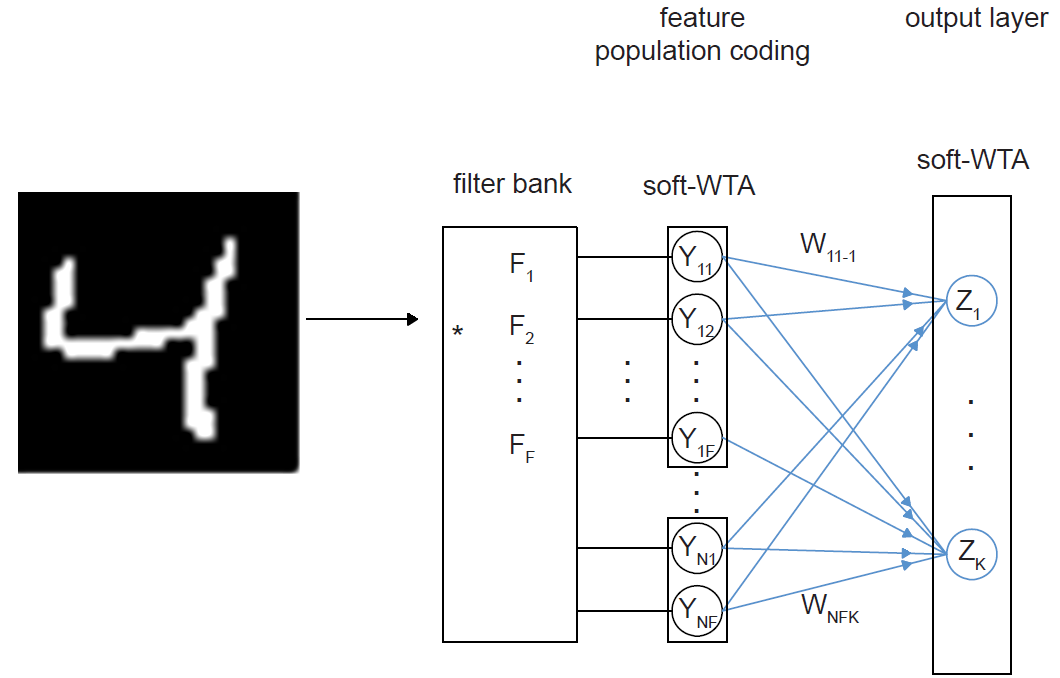
\includegraphics[width=0.8\textwidth]{network_learn_orientations}
\caption{SEM extended with a filter bank and an orientation discriminating WTA circuit for learning an orientation map of a visual stimulus. \label{fig:network_learn_orientations}}
\end{figure}

\begin{figure}[ht]
\centering
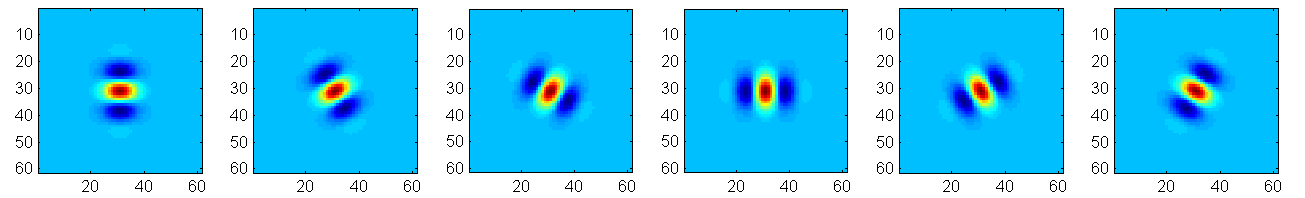
\includegraphics[width=0.8\textwidth]{filters_real}
\caption{Example of Gabor filters (real part). Defined at orientations [0, 150] degrees with increments of 30 degrees. \label{fig:filters_real}}
\end{figure}

The WTA circuits responsible to determine the preferred orientation of all input nodes are activated by convolving the stimulus with a bank of two-dimensional Gabor filters. The filters are defined with different scales and angular orientations from a predefined discrete set. \Cref{fig:filters_real} provides an illustrative example of such Gabor filters. By comparing the magnitude of responses between the filters at each pixel we can decide on the pixel's preferred orientation. Talking about the preferred orientation of a single pixel does not actually carry much meaning. The transformations do yield responses for each pixel but they only become informative in relation to the responses of its neighbors. Examples of filter responses to a binary image stimulus are shown in \cref{fig:response4}

\begin{figure}[ht]
\centering
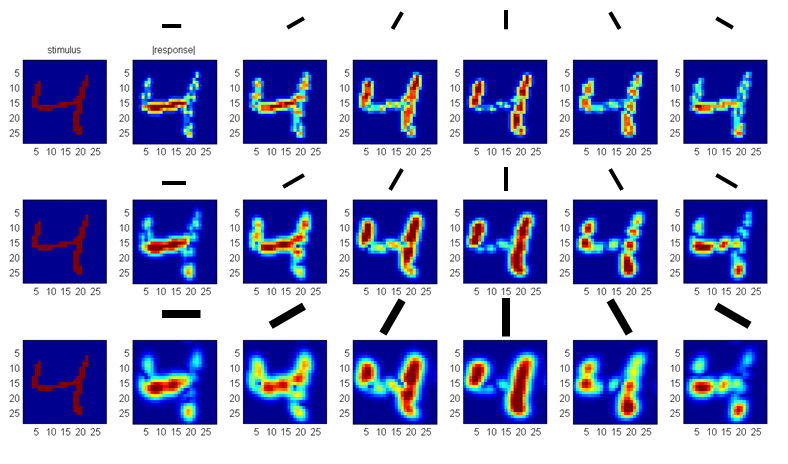
\includegraphics[width=0.8\textwidth]{response4}
\caption{Example of filter response magnitudes when convolving a binary image with Gabor filters defined at different scales and orientations.
\label{fig:response4}}
\end{figure}

Parameterized Gabor functions are an adequate approximation of simple cells in the primary visual cortex \cite{Serre04realisticmodeling, Long2008}. Daugman demonstrates the construction of a neural network to achieve this transformation \cite{Daugman1988}. However, this work adopts the traditional systems' approach for defining and applying the filters.

\subsection{Extending SEM by learning hidden features}

We have seen the computational power of the SEM model as an unsupervised method for identifying hidden causes. So far the hidden causes have been used synonymously with predefined classes (e.g. numerical digits from the MNIST database \cite{LeCun1998}). We extend the SEM model in a way that breaks this assumption. We insert an additional layer, a WTA circuit, responsible for learning hidden causes that depict abstract features of the object we attempt to detect and recognize. This feature layer will contribute to the bottom-up learning as we expose it to the low-level input and and have it drive the WTA circuit already encountered in the original SEM architecture. With this additional feature-WTA circuit introduced, we no longer require presentation of the entire stimulus but will restrict stimulus presentation to subregions within the space of a stimulus. These subregions may represent salient regions within a stimulus. The definition and method of selecting these subregions will be discussed in more detail as we discuss the object detection module.

\section{Object Detection Using Visual Attention}

\subsection{Achieving invariance}

\paragraph{}Itti et. al anchor their bottom-up computational model of attention as a saliency search within a visual scene. They demonstrate how attention is achieved in an image based environment. The image is evaluated for conspicuities in features such as illumination, color, texture or other. The feature extraction is pre-attentive. A spatial map of each feature at different spatial scales is unified into a single conspicuity map for this feature. The conspicuity maps are combined linearly into a saliency map of the image. The saliency map represents a reconciliation of the pre-attentive features as the magnitudes need to be normalized before we can can combine them. The saliency map seeds the search to locate visual objects in a scene. The objects can later be processed for recognition with less computational overheads \cite{Itti2000, Itti2001}.

The above saliency mechanism defines the distribution from which we sample windows of attention. The windows of attention are forwarded to the recognition module as a continuous feed of input. Itti et al. emphasize that their model does not cover any top-down attention components, yet they address the importance of preventing the ``focus of attention from immediately returning to the previously-attended location'' \cite{Itti2000}. This is expected to happen in a purely bottom-up method as the saliency value remains constant. Therefore, we need to bias the model to attend to the second-most likely salient location. Since we are using windows of attention as input to a recognition system, inhibition of return (IOR) enables such input to be more diverse. The proposed mechanism for IOR, adopted from Itti et al is the convolution of the saliency map with a Off-center-On-surround kernel that inhibits the center located on top of the previous window of attention and enhances the saliency of its surroundings. Itti et al. point out that the effect of IOR should remain transient and need only be maintained temporarily \cite{Itti2000}.

\paragraph{}Olshausen et al.'s earlier attempt to formalize a framework for attention includes the concept of bottom-up flow of information before attempting recognition but also mentions the presence of a top-down mechanism intercepting the signal. This mechanism arises from ``control-neurons'' that dynamically modulate synapses, or weights, for routing a selected spatial window from lower levels in the visual system to higher levels \cite{Olshausen1993}. They describe how scale-invariance is achieved through magnification of the window of attention to fit a ``canonical reference window'' \cite{Olshausen1993}. Olshausen's ``canonical reference window'' is also labeled as ``normalization'' by Wiskott in similar context \cite{cogprints3321}. This concept is computationally equivalent to resizing an image via interpolation leading to a blurred appearance of the attended window inside the reference frame. Their control units come into play as they can shift the window of attention up or down scale levels or translate within a single plane, scale. This conscious control represents behavioral control of attention that can arise from motor control. This motor control can be voluntary or not, however the authors are more focused on the case of involuntary control. To demonstrate the employment of the same control neurons as part of a closed-loop autonomous system, Olshousen et al. describe a strategy that governs these control units.
This strategy is made out of:
\begin{itemize}
  \item Low-pass filter the visual scene into blobs.
  \item Point the reference window to the location of the blob, adapting to its topography (i.e. size and location).
  \item Pass the original input represented by the blob to the recognition module.
  \item Assess the matching of the presented object with previously learned objects. Take action according to recognition results (e.g. learn as a new object, discard it, perform a task, etc.) \cite{Olshausen1993}
\end{itemize}
The authors provide an elaborate derivation and description of this model. We see them taking the initial steps of what we learn from Itti's salient-based model in addition to the notion of turning the open-loop system into a closed-loop one through the feedback signal of modulatory control neurons whose activity is a relay of the response of a recognition module. However, we encounter some gaps in how some of the intermediate steps of modulation are defined, as these may depend on application or the recognition module itself, how it operates, how it responds. 

\paragraph{}A computational model of top-down attention is proposed by Baluch et al. The top-down model is described as a mechanism that influences the stimulus drive generated from the familiar bottom-up mechanism. The influences come in the form of feature bias, spatial bias, context or a task being carried out. These same influences can generate an attention field independent of the stimulus drive. The attention field and modulated stimulus drive are multiplied and normalized to yield a response to apply detection on. An analogous top-down attention model is presented that involves a learned approach. A learner is presented with bottom-up derived features to predict top-down saliency. Top-down saliency is multipled by bottom-saliency to form a unified priority map over the visual space \cite{Baluch2011}. This model provides a concise interaction of bottom-up and top-down mechanisms, thus bridging Itti et al.'s with Olshausen et al.'s frameworks.

\paragraph{}The SEM model requires some extensions to achieve scale- and translation invariance. Scale invariance can be achieved through the use of intermediate layers that learn features of visual objects that are more abstract than pixel intensity values. We can predefine these features in the form of orientation maps. It is also possible to let the SEM model learn abstract features driven by the stimuli. The features can be pre-extracted using decimated versions of the orginal visual stimulus, thus reusing existing neurons in the network as if they were with enlarged receptive fields. We expect that these abstract feature nodes can pick up simple shapes such as oriented bars as well as more complex shapes. The network wiring will emerge from the features extracted by the data and the interactions within the stochastic processes of the SEM. The model will become invariant to XY-plane translations through the use of selective visual attenion. Bottom-up saliency-based attention is employed following the model proposed by Itti, Koch and Niebur \cite{Itti2000}. The introduction of a top-down component is discussed as the component may use output-layer spikes as a feed-back signal to modulates attention.

\subsection{Feature-population coding}

Towards invariance to translation we employ Itti et al.'s bottom-up saliency-based attention mechanism. It serves the purpose of locating regions within a visual scene to present to the network. Population coding will be used for encoding an analog and/or binary state of a neuron, $y$ neurons, into spike trains. The state of these neurons will be derived from pixel intensity values, binary, and analog filter responses when convolving salient regions with filters from a predefined filter bank. Population coding derived from filter responses will be referred to as feature population coding. The original simple population coding and feature population coding generate input to a new network whose acrchitecture is illustrted in \cref{fig:architecture_recognition}.

We refer to the original population coding as 'simple' because it operates directly on the bi-state external variable and only generates spikes that elaborate on these two states. The feature population coding investigates the use of a soft-WTA circuit to determine the state of the spiking neuron in a population \ref{fig:network_learn_orientations}. The population represents a set of feature states and the soft-WTA circuit determines the dominant state(s). In this case the population represents the response of a node after convolving the stimulus with a bank of Gabor filters. The WTA circuit draws the preferred orientation from the stochastic process whose distribution is defined by the analog response to each filter. The use of winner-take-all circuits correlates with the HMAX framework \cite{Serre04realisticmodeling, Riesenhuber1999}. Employment of the soft-max operator allows for a representation of intermediate features (i.e. an angular orientation that lies between two predefined states). It also provides good mitigation against local maxima during the learning process.

The bottom-up attention mechanism employed is a varied implementation of Itti et al.'s model. Their model defines a salient-based mechanism to evaluate a visual scene on locations worth attending to.
The commonalities between this interpretation and the original model are:
\begin{itemize}
  \item the use feature maps based on intensity and orientation,
  \item detecting conspicuity from center-surround differences,
  \item normalizing feature conspicuity maps to combine them into a single saliency map.
\end{itemize}
As for differences, unlike the original model, this interpretation:
\begin{itemize}
  \item use feature population coding, Gabor filter transformations with soft-WTA circuits, instead of linear filters,
  \item omits color features, focusing only on binary image stimuli,
\end{itemize}

\subsection{Learning abstract features}

The attention mechanism provides a continuous feed of subregions in the original stimulus space that may contain patterns worth learning for recognizing objects. This can happen whether the attention mechanism is a purely stimulus-driven or modulated by top-down cues. We are willing to restrict the input space used for training and testing the recognition system to patterns that qualify as salient. The SEM model treats such salient windows as its external variables $x$. Population coding, simple and feature-population coding, produces spike trains that represent the intensities in the pixels and their the orientation map of such a window. A layer of $f$ neurons interact within a soft-WTA circuit. These $f$ neurons employ the same learning rule. Their WTA-circuit is essentially the building block brought over from the original SEM model. This layer is described as the abstract feature layer, or $f$-layer, as it learns to discriminate the abstract features provided by the salient window input. The spikes emerging from the $f$-layer activate the $z$ neurons in the output layer. The output layer remains responsible for learning the hidden causes, except that it now discriminates such causes in the distribution of abstract features. It does this with far more reduced dimensionality.

\begin{figure}[ht]
\centering
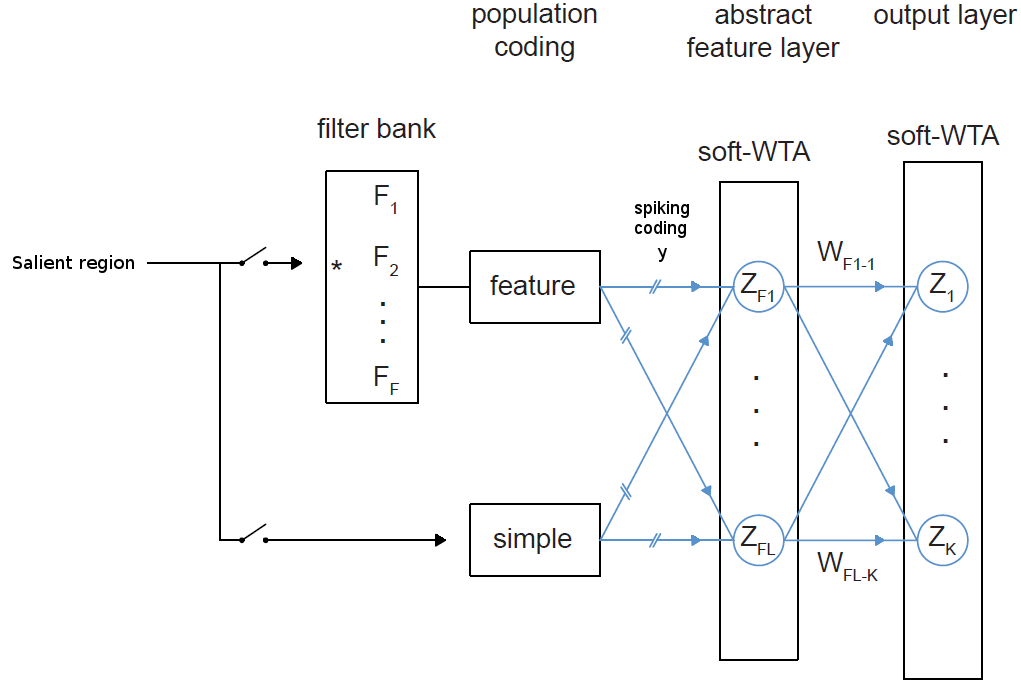
\includegraphics[width=0.8\textwidth]{architecture_recognition}
\caption{The architecture of the recognition module of the extended SEM model. The input is restricted to salient regions provided by the detection module via selective attention. The windows of attention is passed on to population coding, whether simple bi-state coding of pixel intensity values or convolution with Gabor filters and WTA-circuit that discriminates the preferred orientation of the external variables. We will determine if the use of both population coding schemes are necessary or if only one is sufficient. Spikes generated from the population coding activate a soft-WTA circuit in the abstract feature layer, the F-layer. F-layer neurons learn patterns present in the window of attention. The neurons in the output layer learn hidden causes represented by the spiking distribution of the $f$-layer. 
\label{fig:architecture_recognition}}
\end{figure}

\Cref{fig:architecture_recognition} illustrates the wiring of a spiking neural network responsible for recognizing hidden causes in visual objects. The causes are represented by spiking patterns of the output-layer neurons that discriminate the spiking pattern of preceeding neurons in an intermediate layer. Neurons of the intermediate layer respond to the presence of abstract features present in a series of windows of attention. With the presentation of a stimulus a detection module employing selective visual attention generates this series of windows of attention which are encoded into spike trains through population coding. Population coding may be 'simple', based on pixel intensity values, more complex by evaluating the response of the subimage to filters, or both. \Cref{fig:architecture_recognition} reveals this configurability through the placement of switches in front of a population coding module.\\

We recall the use of population coding to encode antagonistic On- and Off-states of a node exciting $z$ neurons. This elaborate representation of the node increases the likelihood of a $z$ neuron detecting correlations, as formulated in \ref{eqn_corr}. We may reuse this technique in elaborating the representation of $f$ spikes exciting $z$ neurons in the output layer. $z$ neurons learn patterns of $f$ nodes firing and not-firing explicitly.\\

Here it becomes necessary to point out a predicament. Attention windows arrive at the recognition module serially. This does not cause any problems for the $f$ neurons as the scope of their operation is within a single window of attention. However, in the case $z$ neurons in the output layer need a larger scope as their response needs to be associated with the original stimulus. 
We may at first look at it as a problem of detecting a temporal pattern. Panchev et. al demonstrate the detection of temporal patterns using spiking neurons. There model is employed in the context of training robots a natural language of instructions. The learning mechanism models dendritic and somatic membrane potentials, thus not restricting itself to only timing information through STDP but also temporal integration of amplitude information. They key takeaway of their work is in achieving a temporal "delay" mechanism and to encode the spatio-temporal structure of the delay mechanism into spikes and have neurons learn such spiking patterns \cite{Panchev2006}. A similar solution to detecting spatio-temporal patterns is demonstrated by Byrnes et. al. Their work abstracts the spatio-temporal patterns as a temporal sequence of symbols. The spiking patterns of neuron reflect the detection of a symbol suceeding the detection of a previous symbol. The preceeding symbol primes the model and this biases the model when the most recent symbol is introduced \cite{Byrnes2010}. This state machine logic aligns well with the problem at hand. To draw an analogy with the model of Byrnes et al. The windows of attention would be represented by symbols and the stimulus would be encoded by the temporal sequence of such symbols. However, our model may not necessarily benefit from learning suc explicit temporal patterns of windows of attention. The presence of symbols is sufficient, yet their temporal order may be negligible. It may suffice to treat the the sequence of symbols $ABC$ the same as the sequence $CBA$, $ACB$ or any permutation of this sequence. Therefore, a solution to this problem is likely to lie in the use of a state machine that models memory and preserves the state of the output layer for different windows of attention belonging to the same stimulus, while remaining invariant to the sequence of such states. We learn that markov chains present a possible approach for maintaining temporal states. Other works dealing with the detection of spatio-temporal patterns also teach us that this may be achieved through the use of self-excitatory synapses for neurons in the output layer. The different ways of approaching this are quite intriguing. We opt for a simple time-delay mechanism:\\

\begin{figure}[ht]
\centering
\includegraphics[width=0.8\textwidth]{time_delay_circuit}
\caption{A simplified abstraction of a time-delayed WTA circuit.
\label{fig:time_delay_circuit}}
\end{figure}

Time-delay components are needed to reconcile attention windows arriving at the recognition module serially. For associating the response of $z$ neurons to a stimulus we employ a time-delay circuit as abstracted by \cref{fig:time_delay_circuit}. The time-delay is represented by associating $f$ neurons with multiple of such time-delayed WTA circuits at the same time. The time-delayed WTA circuits differ in the timing at which they inhibit the $f$ neurons. The number of WTA circuits matches the number of windows of attention sampled from the same stimulus. Effectively this results in superimposing $f$-layer spike trains for each window of attention associated with the same stimulus. Furthermore, this time-delay mechanism effectively discards the temporal information of the sequence.\\

\begin{figure}[ht]
\centering
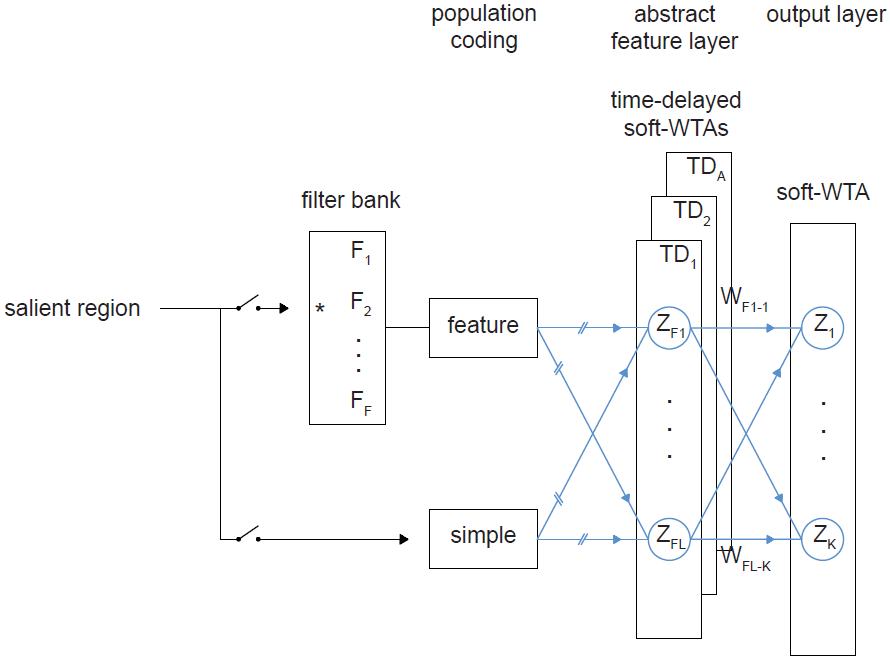
\includegraphics[width=0.8\textwidth]{network}
\caption{The revised network of the recognition module. Input is provided serially by the attention mechanism in the form of windows of attention. Population coding encodes analog intensity or filter response values into spike trains which activate a soft-WTA circuit. Spikes generated from the $z_F$ or $f$ neurons excite $z$ neurons in the output layer. $f$ neurons in the abstract feature layer are responsible for learning and predicting the abstract pattern in the window of attention. The spiking of $f$ neurons is modulated by time-delayed soft-WTA circuits. Each time-delayed WTA is responsible for reconciling the serial arrival of an attention window temporarily and superimposing $f$ spike trains due to that window onto a spike train combining spikes due to all windows associated with the same stimulus. $z$ neurons in the output layer are exposed to spikes due to all windows of the same stimulus simultaneously. They are responsible for learning spiking patterns of the preceding layer associated with hidden causes in the original stimulus.
\label{fig:network}}
\end{figure}

We can now explain the flow of information inside the model illustrated by \cref{fig:network} the following way: Given a stimulus the detection module provides a series of attention window in serial fashion. Population coding represents each window in spike trains that excite learners in the intermediate $f$-layer. For each window of attention a WTA circuit with a delay component inhibits $f$ neurons. This leads to the superimposition of $f$ spike trains due to different windows of attention of the same stimulus. The superimposed $f$-layer spike trains provide excitatory input to $z$ neurons that compete in a soft-WTA circuit and form the output layer of the recognition module.

\subsection{Experimentation}

Prior to presenting results we elaborate on how methods were applied and how the experimentations was carried out. The simulations carried out define the various parameters of the model such as:
\begin{itemize}
  \item Defining the \textbf{dataset} of static image stimuli.
  \item Splitting the dataset into completely separate \textbf{train} and \textbf{test} sets.
  \item Defining \textbf{encoding strategies} of the population coding, such as the encoding frequency of the Poisson process, the sampling rate to treat spike trains as time-series signals, duration of spike trains, enabling/disabling encoding strategies (i.e. simple population coding, feature populating coding, or both as depicted by the switches in \cref{fig:architecture_recognition} 
  \item \textbf{Prediction parameters}: Number of $z$ and $f$ neurons. Whether to train them simultaneously or independently (i.e. simulate the learning of $z$ neurons with pre-learned $f$ neurons)
  \item \textbf{Learning parameters} for either layer: This covers learning rates, initialization of weights, numerical scale and limit of weights, duration of a node's spiking history.
  \item \textbf{Competition parameters} that set the behavior of the WTA circuits: Refractory period for inhibition, parameters for modeling an Ornstein-Uhlenbeck process. Competition parameters may differ between the layers.
  \item \textbf{Feature paramters} relevant for defining feature population coding or defining of pre-attentive features: This involves Gabor function paramters (e.g. filter support radius, number of orientations, orientation resolution, defined scales, frequency and elongation of the gabor kernel.
  \item \textbf{Attention parameters}: Size of attention window, maximum number of attention windows per stimulus (=number of time-delay WTA components)
  \item \textbf{Saliency parameters}: Dimensions of the saliency map and lower threshold values for clipping filter responses that are too low.
\end{itemize}
  
\textbf{Simulation}: The simulations mainly involve:
\begin{itemize}
  \item Constructing a dataset of multiple classes of handwritten digits.
  \item Splitting the dataset into separated train and test partitions.
  \item The procedure of train and test phases of the experiment are identical except that in the train or learning phases weights may be updated. As for the test phase weights remain static.
  \item For each stimulus image:
  \begin{itemize}
  	\item An image is fed into the attention module, which evaluates a saliency map of the stimulus.
  	\item Windows of attention are sampled from a two-dimensional saliency distribution.
  	\item For each window of attention
  	\begin{itemize}
	  	\item The window of attention is encoded into $y$ spike trains.
	  	\item $y$ spikes are fed into time delayed WTA-circuits that modulate the spiking of $f$ neurons
		\end{itemize}
		\item $f$ spikes superimposed by time-delayed WTA-circuits may be re-encoded for more elaborate representation as formulated in \ref{eqn_corr}.
		\item $f$ spikes are fed into WTA-circuits modulating the spiking of $z$ neurons
	\end{itemize}
\end{itemize}
The above procedure is populated with mechanisms for evaluating, logging and observing behaviors such as shape of attention windows, weight updates, spiking patterns, calculating conditional entropy of spiking nodes and measuring computational performance (e.g. speed)\\

\textbf{Evaluation methodology:} For evaluating the impact of configurations in the model we try to follow Nessler et al.'s methodology. Although the SEM model is an unsupervised learning model we make use of the labeled dataset from \cite{LeCun1998} post-learning. The evaluation methods involve calculating firing probabilities of $z$ neurons given the presentation of a particular class (e.g. $p(z=1|c=C)$). Or measuring the conditional entropy of firing. For the original SEM model, the success of an experiment was measured in how low conditional entropy and how fast it declined, as this reflected the specialization of a learner to a particular class \cite{Nessler2010}. As we extend the SEM with an additional layer of abstract features, we do not expect conditional entropy to behave the same way. We do not state expectations on the distribution of $f$ or $z$ neurons to a particular class. It is almost meaningless to do so for $f$ neurons since they are originally intended to learn generalized patterns that span across different classes. Therefore we allow for a many-to-many relationship. We may observe $f$ neurons specialized to a pattern that is present in a single class (low entropy), we may also encounter an $f$ neuron learning a generic shape observed in multiple classes (high-entropy). We continue relying on the firing probability distribuitions of the spiking learners in either layer given a stimulus class. The measure of evaluation will be in the uniqueness of such probabiliities, so that we may conclude that each class may be represented by a distinct firing patterns that enables successful recognition. The uniqueness may be measured by the euclidian distance of two multi-dimensional distributions given two different classes $D(c_i, c_j)$ as formulated in \ref{eqn_eval_distance}.

\begin{equation}
		D(c_i, c_j) = D(c_j, c_i) = \sqrt{\sum_{k=1}^{K} [c_i(k)-c_j(k)]^2} \\
	\label{eqn_eval_distance}
\end{equation}
where
\begin{itemize}
	\item $i$, $j$ denote a class of set of classes $c$,
  \item $c_i$ denotes the firing probability distribution of a learner given class $i$,
  \item $k$ denotes the dimension or index of the learner within the distribution, while $K$ denotes the space of learners whose firing probabilities form the distribution $c_i$ and $c_j$.
\end{itemize}

A more sophisticated and appropriate measure for measuring difference between probability distributions is provided by the Kullback-Leibler (KL) Divergence. The symmetric KL divergence is defined as $D_{KL}(c_i||c_j)+D_{KL}(c_j||c_i)$ where $D_{KL}(c_i||c_j)$ is defined in \ref{eqn_eval_kldiv}:

\begin{equation}
		D_{KL}(c_i||c_j) = \sum_{\substack{
																	   k=1 \\
																	   c_i(k) \neq 0 \\
																	   c_j(k) \neq 0
																	  }}^{K} c_i(k) \ln{\frac{c_i(k)}{c_j(k)}}  \\
	\label{eqn_eval_kldiv}
\end{equation}
where distributions $c_i$ and $c_j$ sum up to 1 \cite{Kullback1951}.

\chapter{Results}

\section{Exploiting inherit noise of a stochastic process for handling missing values}

The first extension to the SEM network was to enrich the representation of the external variables $x$. Instead or in a addition to bi-state pixel values we convolve the image input with a set of Gabor filters. A WTA-circuit is applied to the response of each pixel to the Gabor filters to determine its preferred orientation through a stochastic process. The use of the stochastic process is not as noise-free as applying $argmax(y_i)$, where $y_i$ denotes the magnitude responses of pixel $i$. The $argmax$ operator would even align well with the HMAX paradigm presented in the works of Riesenhuber, Poggio and Serre \cite{Riesenhuber1999, Riesenhuber2000, Serre04realisticmodeling, Serre}. However we have find that noise inherit in the stochastic process mitigates the computational pitfall of low magnitdue response vectors very well. To elaborate, parts of the stimulus with very low intensity values, will result in low magnitude response values for all filters in the filter bank. Nessler et al. refer to this as "missing values" \cite{Nessler2013}. However, the insignificant response vector for a pixel still yields a result from the $argmax$ operator. It will actually yield a near constant result. To avoid learners from learning this constant pattern that does not carry any true information, we need a mechanism to handle such low response values. The problem is not really in the response vector of all-low magnitudes. We can generalize the problem to pixel response vectors with high uniformity. We can still align this model with the HMAX model if we resort a stochastic process. The stochastic process is able to resolve high-uniformity, high entropy, distribution of pixel response vectors through its inherit noise. If a learner relies on such response vectors as weights, the spike trains coding the response vector will reflect the uniformity and the learning rule will yield accordingly uniform weight distributions for the corresponding pixel, leaving such weights computationally useless. We find that the weight vector associated with this pixel is as uniform as the response, thus with the use of a soft-WTA the contribution of this vector of weights for this pixel relative to the global weight vector of the learner is merely constant. Thus the membrane potential of this neuron will not experience fluctuations due to these weights but rather weights whose local vectors have low entropy. \Cref{fig:weightsPerOrientation} depicts the distribution of weights associated with different orientations after a learning process involving handwritten digits as stimuli. We find that outer areas with generally low intensity activity are high regardless of orientation.

\begin{figure}[ht]
\centering
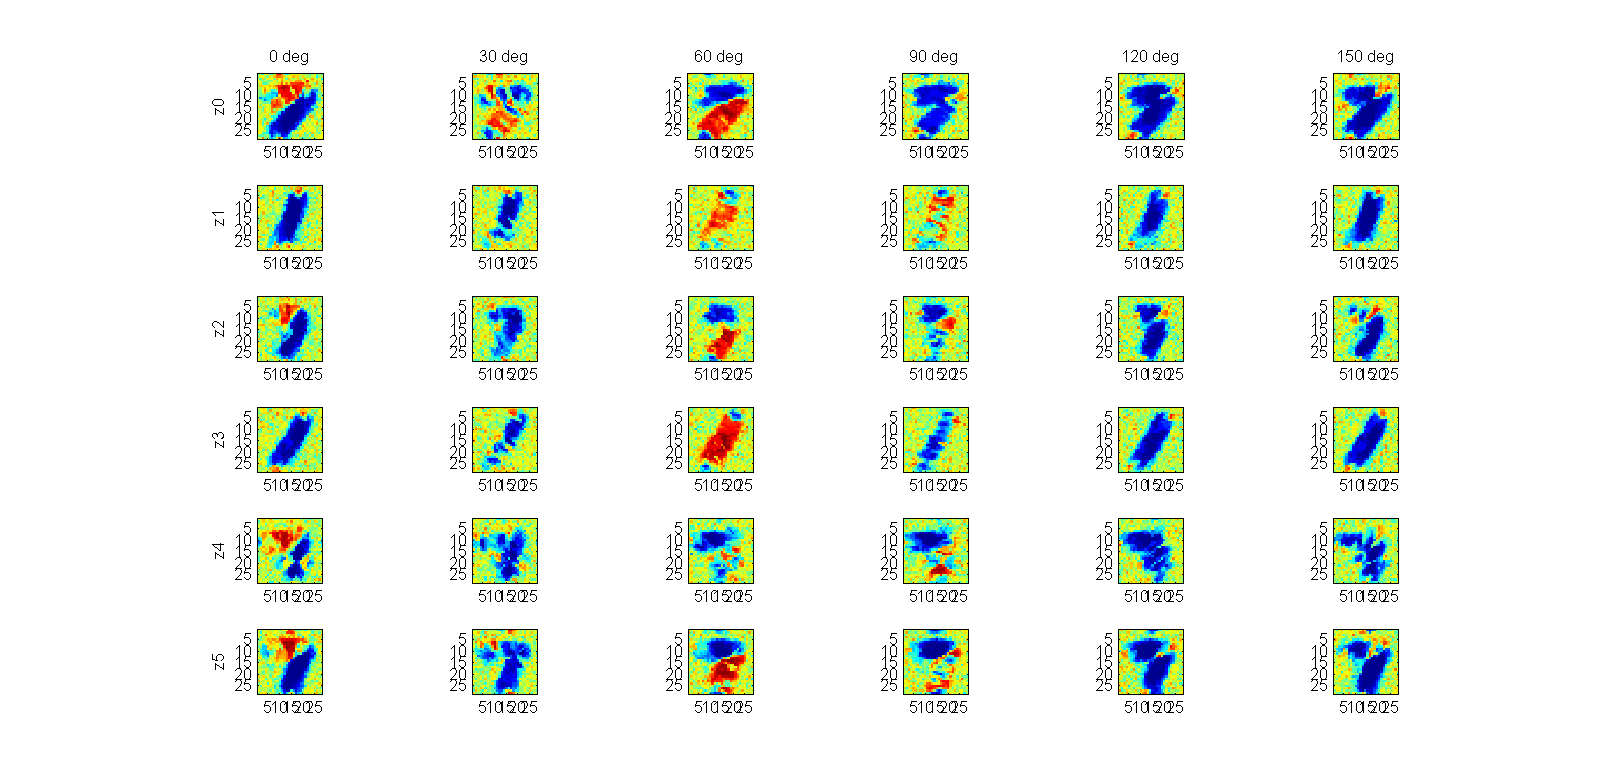
\includegraphics[width=1.2\textwidth]{weightsPerOrientation}
\caption{Example of $z$ neuron weight distributions for different orientations when using while utilizing a stochastic process for handling missing values and accounting for the uniformity of a pixel's response. Each row of subplots is reserved for a learner $Zi$, while each column is associated for an orientation. This is from an experiment involving handwritten variants of the digits 1 and 7 \cite{LeCun1998}. Blue colored regions have low weight values that yellow, orange and red, represent strong weights.
\label{fig:weightsPerOrientation}}
\end{figure}

If we picked the same weight from each orientation for the same learner, we'll find the distribution of this local weight vector to be fairly uniform. A local weight vector belonging to a pixel in an active region, will have some very low weight values for most orientations, and very high weight values for fewer. \Cref{fig:weightCondEntropy} accomplishes this. It generates a local weight vector for each pixel, calculates its entropy to visualize the non-uniformity of the weights associated with each pixel in the XY-plane. Stimuli that activate weights belonging to a local weight vector with high netropy are a mere DC component in the resulting membrane potential of a neuron. While changing the input that invokes activity in weights belonging to low-entropy local distribution, will yield significant changes in that same neuron's membrane potential. \Cref{fig:weightMaps47_masked} provides a more compact visualizations of the weight distribution by indicating the dominant weight, or preferred orientation associated with each external variable $x$ for different neurons $z$.

\begin{figure}[ht]
\centering
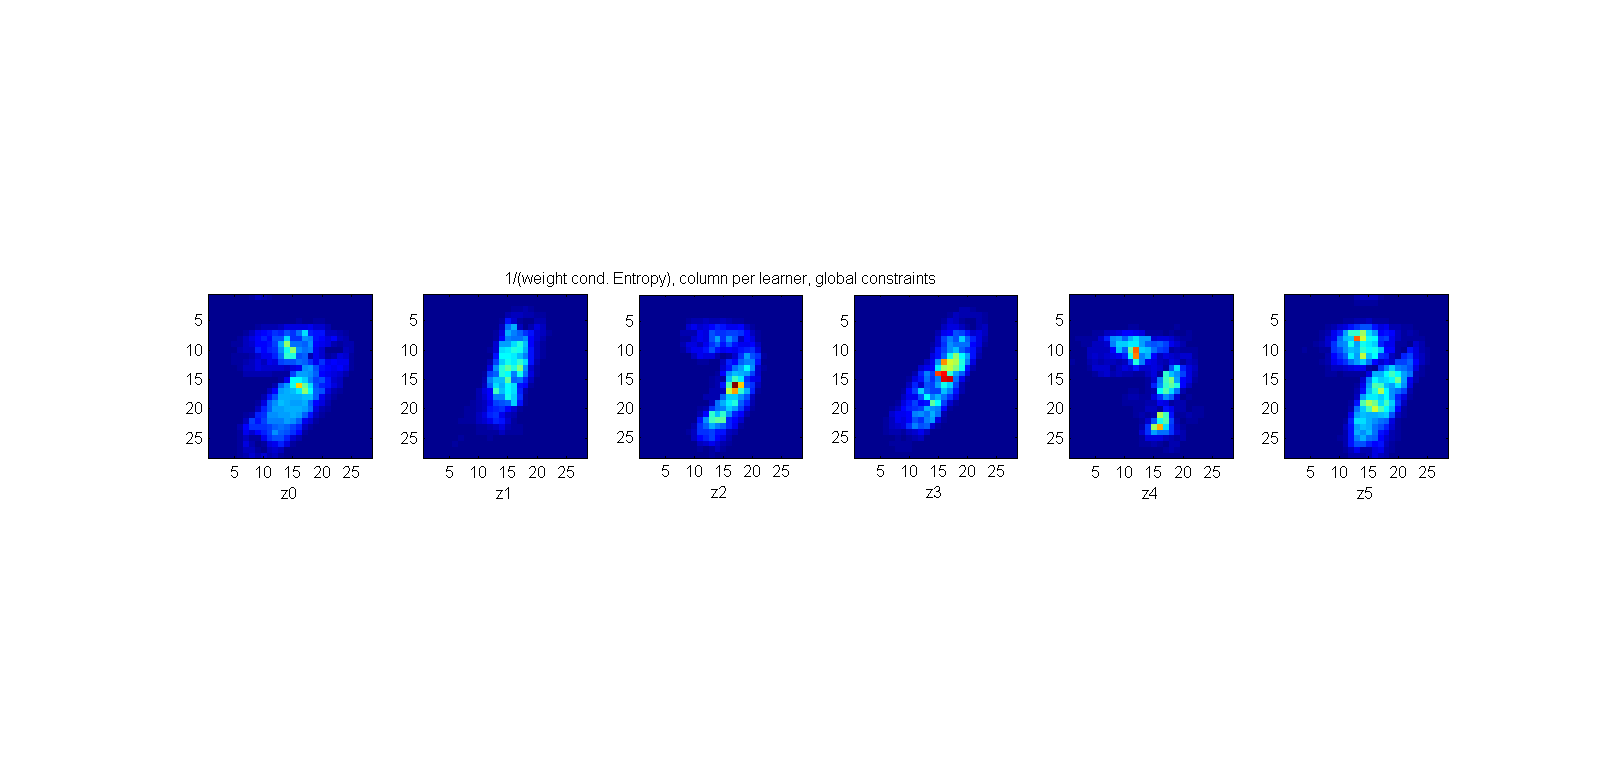
\includegraphics[width=0.8\textwidth]{weightCondEntropy}
\caption{Entropy of local weight vectors representing orientations associated with the same pixel. The intensity values in the image are anti-proportional to the entropy of the pixel's weight vector. This is from an experiment involving handwritten variants of the digits 1 and 7 \cite{LeCun1998}. Bright intensities are associated with low-entropy, strongly discriminating weight vectors, while low intensities are associated with uniform weight vectors whose contributions are merely DC components to the neuron's membrane potential. Each image represents this non-uniformity distribution of different learners.
\label{fig:weightCondEntropy}}
\end{figure}

\begin{figure}[ht]
\centering
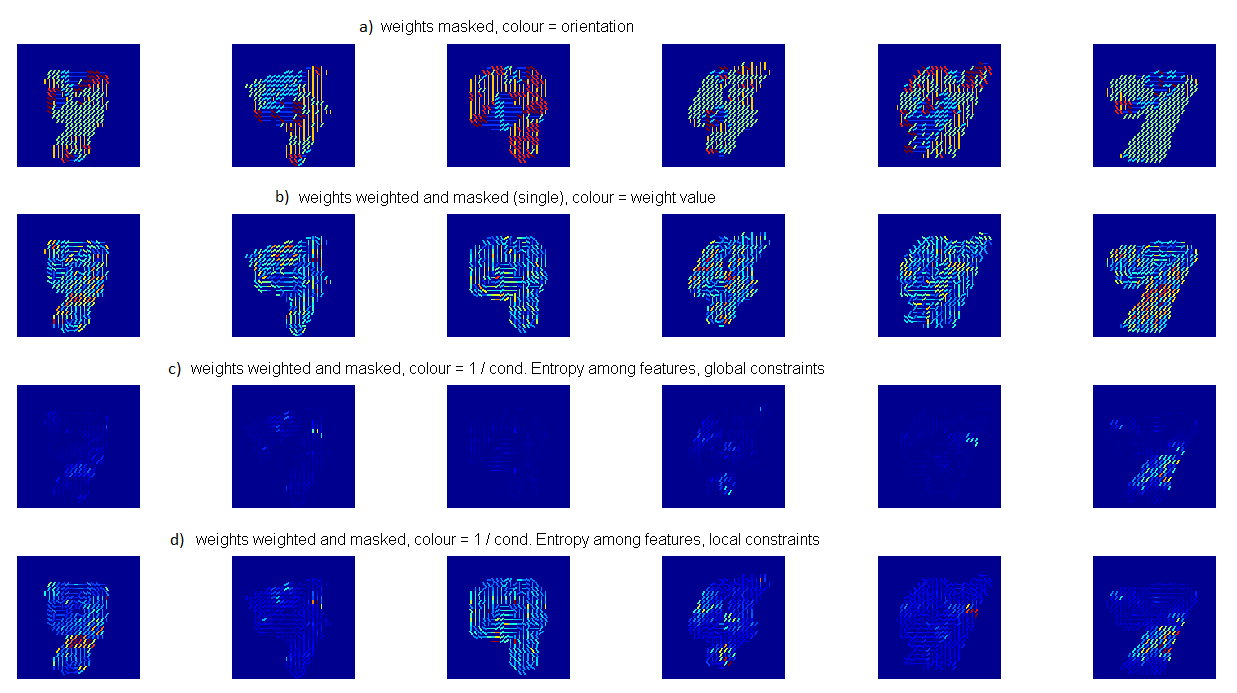
\includegraphics[width=1.2\textwidth]{weightMaps47_masked}
\caption{Visualizing weights of $z$ neurons after learning orientation maps of handwritten digits. Data used: a subset of handwritten digits from the MNIST database (classes 7 and 4) \cite{LeCun1998}, no overlap between training and test sets. Each column of images belongs to a $z$ neuron. The weight weight vectors have been reduced to two dimensional matrices by finding the dominant weight for each pixel. The preferred orientation of each pixel is determined via $argmax(\textbf{w}_x)$ where $X$ refers to the pixel and $w$ is the weight vector associated with this pixel. The length of \textbf{$w$} is proportional to the number of possible orientations defined. Regions of the image with very low intensity activity have been masked and appear plain while color represents  \textbf{a)} the preferred angular orientation of a pixel, \textbf{b)} the magnitude of the weight of the preferred orientation, \textbf{c)} the non-uniformity of a weight vector \textbf{$w_x$} normalized across all learners and \textbf{d)} the non-uniformity of a weight vector \textbf{$w_x$} normalized across the image. 
\label{fig:weightMaps47_masked}}
\end{figure}

\section{Measuring Saliency using feature-population coding}

Saliency is measured with the use of feature maps, one for intensity features and a second for orientation features. The intensity feature map is generated by convolving the stimulus with a Difference of Gaussians for achieving centre-surround operations. Normal localization is applied on the filter response to empahsize conspicuities and a global normalization is applied on the entire feature map for later reconciling this itenstiy contrast map with other feature maps.  
The same stimulus is convolved with bank of Gabor filters. For each pixel the filter responses for that pixel are taken as input to a soft-WTA circuit. The soft-WTA circuit determines the preferred orientation of the pixel. Performing this for all pixels we generate an a map of the preferred orientation for each pixel, an orientation map. In order to detect conspicuities in these orientations we measure the distance of a pixel's preferred orientation relative to its neighbors and use the local variance of these diatance measures as a measure of concpicuity in orientation. The feauture map is then normalized globally and then masked for nodes with low magnitude responses to all filters before its use alongside the intensity contrast map.
The intensity contrast and orientation conspicuity maps are combined linearly into a single saliency map. Nodes in the saliency map with high response-magnitude indicate either high contrast, orientation conspicuity or both. The saliency map serves as a two-dimensional distribution from which we draw coordinates of locations worth attending to. \Cref{fig:saliency_examples} depicts examples of saliency maps evaluated for static images.

\begin{figure}[ht]
\centering
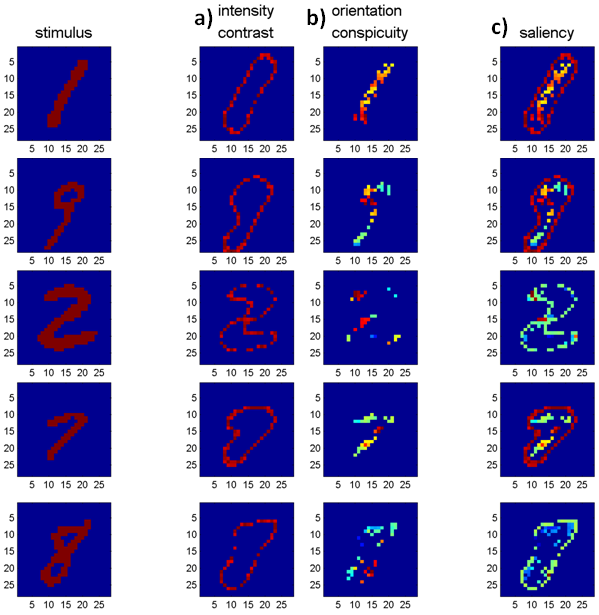
\includegraphics[width=0.8\textwidth]{saliency_examples}
\caption{Examples of saliency maps generated from handwritten digits from the MNIST database \cite{LeCun1998}, where columns depict \textbf{a)} intensity contrast; response to convolving stimuli with a Difference of Gaussians kernel, \textbf{b)} orientation conspicuity; local variance of a pixel's preferred orientation relative to neighboring pixels, \textbf{c)} stimulus map of input stimuli; linear combination of intensity contrast and orientation conspicuity.
\label{fig:saliency_examples}}
\end{figure}

The selection of the attention window is determined through a stochastic process. This non-deterministic process may mitigate the problem of locking onto the same region during successive sampling events, thus increasing the chance of delivering more diverse information to the recognition system. 

\begin{figure}[ht]
\centering
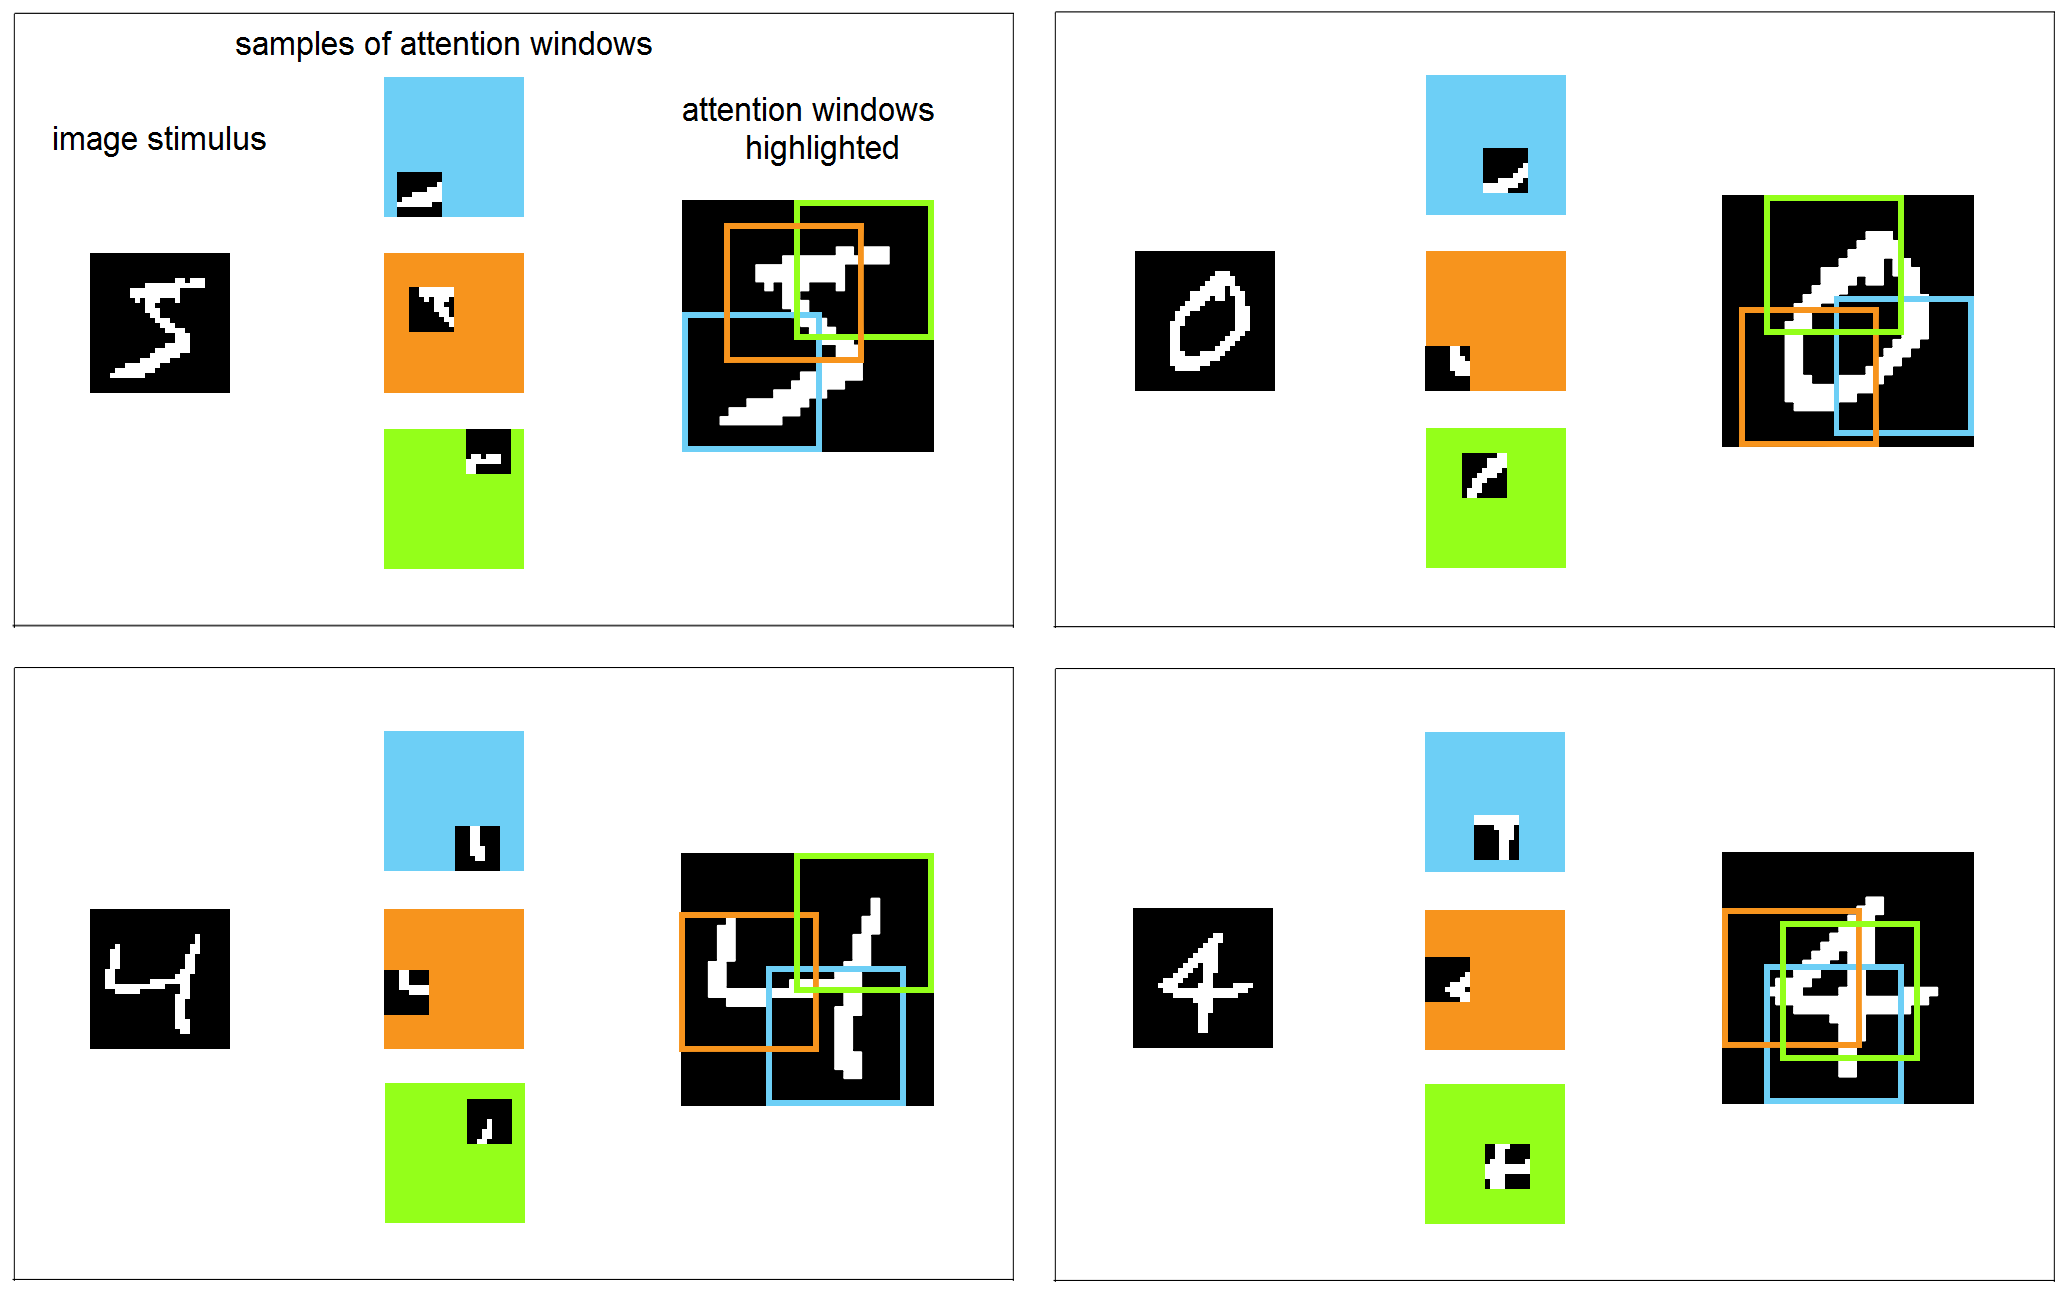
\includegraphics[width=1.2\textwidth]{attention_windows_examples}
\caption{Examples of attention windows determined by sampling from a two-dimensional saliency distribution.
\label{fig:attention_windows_examples}}
\end{figure}

\section{The $f$-layer}

The injection of an intermediate layer with excitatory synapses to $z$ neurons in the output layer provides a reduction of dimensionality for these neurons and exploits the input provided from the attention mechanism. Dimensionality reduction through introduction of hierarchies has been claimed an ingredient towards constructing deep-belief networks \cite{Hinton2006}. This layer is mainly concerned with learning abstract geometrical shapes based on low-level features such as intensities and orientation maps.\\

\begin{figure}[ht]
\centering
\includegraphics[width=0.8\textwidth]{architecture_model}
\caption{Block diagram of extended SEM model.
\label{fig:architecture_model}}
\end{figure}

\Cref{fig:architecture_model} illustrates a high-level diagram of the extended SEM model and dissection of a stimulus into windows of attention for performing recognition. In order to reconcile the arrival of attention windows serially and the need of presenting $z$ neurons with $f$ layer spikes representing the entire stimulus and not just individual windows, we employ a separate WTA-circuit onto $f$ neurons for each window of attention, thus introducing a delay of the $f$ spikes due to a particular window. This delay is inversely proportional with the the order of the window's arrival. It effectively discards the temporal ordering of windows and presents the $z$ neurons with a spike patterns that are invariant to the order the windows were evaluated in.\\

The extended SEM network up to and including the $f$-layer is essentially a network for discriminating hidden causes using intensity and orientation features, while restricting the size of the learning nodes' receptive fields.\\

\begin{figure}[ht]
\centering
\includegraphics[width=1.2\textwidth]{response_n_label_all_classes}
\caption{Simulation traces. a) Raster plot of class labels during training phase (dataset composed of digits 0-9). b) Raster plot of $f$-layer spikes. c) Raster plot of output layer spikes. d) Line plots of membrane potential $u$ for output-layer nodes $z$. Each line represents a $z$ neuron. d) Heat map of membrane potential $u$ for output-layer nodes $z$. A projection of d) onto the XZ-plane. Each row in the heat map represents $u$ of a single neuron $z$. All plots are vertically aligned.
\label{fig:response_n_label_all_classes}}
\end{figure}

The computational capabilities of the extended SEM at recognizing visual objects can be demonstrated with reference to \cref{fig:response_n_label_all_classes}. The illustration demonstrates a raster plot of class labels which are available but are kept unused during the training process as this is an unsupervised model. Additionally we see the raster plots spikes of $f$ and $z$ neurons as well as line plots of $z$ neurons' membrane potentials $u$. The membrane potentials are also visualized as a heat map. Unlike raster plots provided by Nessler et al. We no longer recognize the firing patterns visually. Learners have become responsive to more complex distribution patterns that vary in uniformity, unlike low-entropy spiking patterns found in the original SEM model \cite{Nessler2010}. Still, we see neuron-specialization taking place as vertical uniformities in response and membrane potentials degrade with time.\\

A visual aid for assessing simulation results is in visualizing the receptive fields of the spiking nodes. A simple technique for this is Spike-triggered average (STA). To view the average stimulus preceding a spike for each learner, we traverse the spike train of each learner and accumulate a sum of the external variables that have induced a spike. For this exercise we neglect the neurons' accumulation of a history window. The accumulated sum of external variable is divided by the number of spikes, yielding the average stimulus. As we preserve the spatial arrangement of external variables we can visualize the STA as an image. For $f$ neurons the dimensions of this image correspond to the dimensions of the attention windows. For $z$ neurons the dimensions match those of the original stimulus. \Cref{fig:masks_layerF_all_classes_no_singles} illustrates an example of STA for representing the receptive fields of the $f$ neurons, while \cref{fig:masks_layerZSub_all_classes_no_singles} illustrates this for $z$ neurons. We find the STAs of $z$ with few if not any contrast for identifying which class a $z$ neuron prefers. \Cref{fig:masks_layerF_all_classes_singles} and \cref{fig:masks_layerZSub_all_classes_singles} provide an addiotnal view of neuron STAs with samples of spike inducing stimuli. Looking at \cref{fig:masks_layerZSub_all_classes_singles} we need something to verify the internal models of the $z$ neurons.

\begin{figure}[ht]
\centering
\includegraphics[width=0.8\textwidth]{masks_layerF_all_classes_no_singles}
\caption{Examples of STA for $f$ neurons. Optimal simulation conditions chosen for assessing upper bounds for such visualizations.
\label{fig:masks_layerF_all_classes_no_singles}}
\end{figure}

\begin{figure}[ht]
\centering
\includegraphics[width=0.8\textwidth]{masks_layerZSub_all_classes_no_singles}
\caption{Examples of STA for $z$ neurons. Optimal simulation conditions chosen for assessing upper bounds for such visualizations.
\label{fig:masks_layerZSub_all_classes_no_singles}}
\end{figure}

\begin{figure}[ht]
\centering
\includegraphics[width=0.8\textwidth]{masks_layerF_all_classes_singles}
\caption{Examples of STA for $f$ neurons with individual samples of spike inducing stimuli. Optimal simulation conditions chosen for assessing upper bounds for such visualizations.
\label{fig:masks_layerF_all_classes_singles}}
\end{figure}

\begin{figure}[ht]
\centering
\includegraphics[width=0.8\textwidth]{masks_layerZSub_all_classes_singles}
\caption{Examples of STA for $z$ neurons with individual samples of spike inducing stimuli. Optimal simulation conditions chosen for assessing upper bounds for such visualizations.
\label{fig:masks_layerZSub_all_classes_singles}}
\end{figure}

In addition to using STA for visualizing receptive fields, we can look directly at the $f$ neurons' weight vectors \textbf{$w$}. \Cref{fig:weights_pl_pf_intensity} provides us with a visualization of weights of synapses encoding intensities. Intensity coding synapses are two-fold, a synapse for learning the pixels Off-state and a second for learning the pixel's Off-state. A more compressed visualization of this, would be to apply an $argmax$ operator for the two synapses associated with each pixel like in \cref{fig:weights_pl_intensity}. While we use visibility over the actual weight values, we still get a sense of the neuron's receptive filed.

\begin{figure}[ht]
\centering
\includegraphics[width=0.8\textwidth]{weights_pl_pf_intensity}
\caption{Receptive fields of $f$ neurons by visualizing weights of synapses encoding pixel intensity states (i.e. Off-state and On-state). Each sub image is the receptive field of an $f$ neuron.
\label{fig:weights_pl_pf_intensity}}
\end{figure}

\begin{figure}[ht]
\centering
\includegraphics[width=0.8\textwidth]{weights_pl_intensity}
\caption{Receptive fields of $f$ neurons by compressing weights of synapses encoding pixel intensity states via the $argmax$ operator. This yields the preferred state for this pixel. Each sub image is the receptive field of an $f$ neuron.
\label{fig:weights_pl_intensity}}
\end{figure}

Doing the same for $z$ neurons would not be as illustrative as the weights correspond abstract features. We have seen that STAs of $z$ neurons are not very informative. We could visualize the $z$ neurons receptive field by cascading the receptive fields of $f$ neurons. By keeping track of the spatial alignment of attention windows that result in an $f$ neuron firing we would be able to reconstruct an cascade of such windows. We may look at this as an STA of local windows. \Cref{fig:attention_windows_examples} is an example of such a reconstruction mechanism with a minimal number of sample windows and stimuli. 

In order to assess the computational value from the simulation data we resort to evaluating the probability distributions of spiking nodes in the presence of distinct classes. It is worth inspecting such distributions resulting from simulations that use a larger number of learners for either layer. \Cref{fig:prediction_stats_heat_layerZ} provides a comprehensive outlook on prediction statistics generated from a simulation. This particular simulation included samples from all classes of digits [0, 9]. We notice that learners no longer acquire low conditional entropy as expected in the original SEM model. An alternative measure of distribution divergence is illustrated in \cref{fig:prediction_stats_kl_layerZ_0-9}. From this we get a sense of how the recognition of a class is coded in the spiking pattern of the $z$ neuron and how unique the signature for each class is. We may inspect this visualization of firing probabilties for $f$ neurons. In the case of the $f$-layer it is common to find on or more nodes that represent the two opposite extreama. A node with very non-uniform distribution of firing probabilities for the various classes. This node is responsible for predicting an abstract pattern that is unique for a particular class. On the other hand we encounter firing probabilities with high uniformity and this emerges from neurons specializing for a pattern that is generic and present in multiple classes. \Cref{fig:firing_prob_klDiv_layerF_0to9} depicts illustrations of such distributions for $f$ neurons. It may also occur if a class has multiple highliy varying forms. an example of this would be the different ways of writing the digit 7, confirming observations made for the original SEM model \cite{Nessler2010}.\\

\begin{figure}[ht]
\centering
\includegraphics[width=1.3\textwidth]{prediction_stats_heat_layerZ}
\caption{Prediction statistics for $z$. (a) cnoditional entropy of a classes, (b) heat map of conditional firing probabilities of learners, (c) sorted distribution of a conditional firing probabilities, (d) distance matrix for measuring divergence between distributions, (e) conditional entropy learners 
\label{fig:prediction_stats_heat_layerZ}}
\end{figure}

\begin{figure}[ht]
\centering
\includegraphics[width=0.8\textwidth]{prediction_stats_kl_layerZ_0-9}
\caption{KL-divergence of firing probability distributions for $z$ neurons for various classes. As the conditional entropy is becoming less indicative we evlaute the model based on the presence of distinct distributions of classes in the learners.
\label{fig:prediction_stats_kl_layerZ_0-9}}
\end{figure}

\begin{figure}[ht]
\centering
\includegraphics[width=0.8\textwidth]{firing_prob_klDiv_layerF_0to9}
\caption{Heat map of conditional firing probability distributions for $f$ neurons (left). KL-divergence of the classes' firing probability distributions.
\label{fig:firing_prob_klDiv_layerF_0to9}}
\end{figure}

We recall the discussion of \cref{fig:architecture_recognition}, where we point out that the $f$ layer may be configured to receive spikes which encode intensity variables, feature variables or both. So far we have seen receptive responses and receptive fields of $f$ neurons receiving intensity encoding spikes. \Cref{fig:weights_orient_layerF}. In order to investigate the impact of different configurations. A simulation is run for the remaining configurations. \Cref{fig:response_n_label_all_classes_lowFiringRate} demonstrates the outcome of a simulation where $f$ neurons rely only on spikes generated from feature population coding. It is visible that inspite of the large dataset the firing activity of all learners appears insignificant. The suspicion arose that the firing rate of feature population coding was not compatible with the learning rate of the $f$ neurons. However it turns out that the problem was due to insignificant filter response magnitudes. Gabor filter kernels were defined according to the dimensions of the attention windows which were too small yielding a compromised kernel definition.

\begin{figure}[ht]
\centering
\includegraphics[width=0.8\textwidth]{weights_orient_layerF}
\caption{Receptive fields of $f$ neurons by compressing weights of synapses encoding preferred orientations of pixel's via feature population coding. The color depicts an orientation angle. Each image column denotes the receptive field of an $f$ neuron. The rows differ in the masking of missing values. The top row masks units with very small magnitudes, while the second row masks the weight matrix by multiplying it with the neurons STA.
\label{fig:weights_orient_layerF}}
\end{figure}

\begin{figure}[ht]
\centering
\includegraphics[width=1.2\textwidth]{response_n_label_all_classes_lowFiringRate}
\caption{Simulation traces. a) Raster plot of class labels during training phase (dataset composed of digits 0-9). b) Raster plot of $f$-layer spikes. c) Raster plot of output layer spikes. d) Line plots of membrane potential $u$ for output-layer nodes $z$. Each line represents a $z$ neuron. d) Heat map of membrane potential $u$ for output-layer nodes $z$. A projection of d) onto the XZ-plane. Each row in the heat map represents $u$ of a single neuron $z$. All plots are vertically aligned. This simulation is uses an identical configuration as the simulation in \cref{fig:response_n_label_all_classes}, except that it used a richer dataset and that it relied solely on feature population coding. The low firing activity is attributed to Gabor filter kernels being defined with image dimensions that were too small for yielding informative responses.
\label{fig:response_n_label_all_classes_lowFiringRate}}
\end{figure}

For assessing the extended SEM model's robustness to translated stimuli, we induce translation artifacts into the existing dataset and observe the divergence of firing probability distributions between a reference model and a test model. The reference model has only seen data in its original form \cite{LeCun1998}. If we look at the individual samples in this data we may find that the objects are reasonably centered. The slight shift of the object in the XY-plane is expected and may have happened in the recording process. We do not consider these shifts to be significant translations. The reference model undergoes the training and testing phase. We will use the statistics obtained from the testing phase as a reference for comparison.\\
Before executing the simulation on the test model, we generate a revised dataset using the original data while inducing random translation artifacts that place the original object onto a larger canvas. The translations are drawn from a uniform distribution. We reduce the revised dataset to a single class. The model is configured to cope with the new dimensions of the stimulus, these settings will propagate into the relevant internal components such as the filter kernels. However, we will ignore the learning phase and proceed to the test phase immediately. The weights of the learners will be initialized with weight vectors obtained from the reference model. This experiment investigates if a model that has no notion of translated objects will produce spiking patterns that are similar to the reference. This assesses the invariance to translation. The attention module is essentially the only component that has to cope with the translations. The recognition system is unaware of these altered circumstances. \\
The assessment scale invariance uses the same methodology, by utilizing the learner weights of the reference model and running through the testing phase of a simulation while exposing the model to scaled versions of the stimuli.\\
\Cref{fig:comparison_of_cond-prob-distr_tns-layerF-and-layerZ} shows the conditional probability distribution of firing activity of $f$ and $z$ neurons. In order to quanitfy similarities between these distributions we compute the KL-divergence between the three variants of the model. \Cref{fig:KLDiv_ts_layerF-and-layerZ} visualizes the divergence of the probabilty distributions. First we see the KL-divergence of neurons' firing probabilites for the different classes to get a sense of how specialized the neurons are. The class that was used for these experiments is present in this set. The lower plots illustrate the divergence of the firing patterns for $f$ as well as $z$ neurons given a common class while varying the experimental condition (i.e. original unaltered stimulus as reference, exposed to stimuli with translation artefacts, exposed to stimuli with translation and scale artefacts). As the upper and lower KL-dvergence matricies share the same heat intensity scale, we may visually compare that the model when exposed to the artefacts emits spiking patterns that don't deviate to the extent of confusing the firing pattern with a different class. However, there is divergence for the same class after having induced artefacts into the stimuli. The divergence is less for the $f$-layer than the output layer. The divergence increases with adding the scale artefact ontop of the translation artefact.

\begin{figure}[ht]
\centering
\includegraphics[width=1.0\textwidth]{comparison_of_cond-prob-distr_tns-layerF-and-layerZ}
\caption{Comparison of conditional firing probability distributions of learners, $f$ and $z$, between a reference model and test models that utilize what the reference model has learned while exposing them to translated and scaled variations of the original stimuli of a single class.
\label{fig:comparison_of_cond-prob-distr_tns-layerF-and-layerZ}}
\end{figure}

\begin{figure}[ht]
\centering
\includegraphics[width=0.8\textwidth]{KLDiv_ts_layerF-and-layerZ}
\caption{KL-divergence of firing probability distributions for $f$ neurons (left) and $z$ neurons (right). The upper divergence matrices illustrate the measure of distances of two neurons' distributions given the same class. The lower half of the plot illustrated the KL-divergence pf probability distribution after exposing a trained model to stimuli with translated and scaled artifacts. The divergence is calculated between the model exposed to these artifacts and the reference model that was used for training the learners and was only exposed to unaltered stimuli. Vertically aligned heat maps share the same intensity scale.
\label{fig:KLDiv_ts_layerF-and-layerZ}}
\end{figure}

\chapter{Discussion and Conclusion}

The original SEM model is extended to acquire the ability to recognize objects regardless of their position in the XY-plane or their appearance in difference scales on the same plane. This invariance was established through a modular architecture. The model is composed of a detection model governed by visual attention. The module has no concept of the objects it detects, it detects them based on their salient appearance in the visual scene. The second module is responsible for recognition. The recognition module is passive in that it is fed visual stimulus and learns to discriminate the hidden causes it finds in them. The recognition modules, especially in this purely bottom-up, feed-forward, topology of the system, has no influence over the detection module providing it with visual input. The bottom-up framework inspired by Itti et al. faciliates the modularity of the architecture. Modularity provides some conviences when experimentation and prototyping as we keep components fixed while we tune others.\\
In spite of modularity and independence of the detection and recognition modules, we observe that invariance did not emerge solely from attention alone. The use of feature population coding and the injection of an intermediate layer of learners for learning abstract data-driven features, contribute significantly to this. The feature population coding serves the purpose of providing a richer feature representation than intensity alone. We have seen it benefit the recognition module and lowering firing entropy, thus enabling neurons to create more distinct internal modules of objects, with no need for more data and longer training experiments.

The $f$-layer may be the most effective extension to the SEM model as it integrates in such an intriguing way. The $f$-layer is made out of all the building blocks we have encountered in the original SEM model. It accepts spiking input from population coding, it a network of learners in a WTA circuit and population coding again which is applied on it to facilitate higher correlations for successive layers. Here population coding serves the purpose of a increasing the layer's fan out, since its nodes are already spiking. By learning abstract shapes $f$ neurons in the same layer may play roles of simple cells as well as complex cells. That they exist in the same layer and are governed by the same WTA circuit is not intuitive from a biological standpoint when we think of the hierarchies in the visual system. This may put the biological plausibility of the how the layer is situated within the model into question. A thought that arises from this, is that since there are no restrictions that promote any particular complexity of the shape that an $f$ neuron learns, there should not be a distinction in how complex or simple they are. It may even be expected for these varying complexities to arise considering how few layers we have in the network. Hence $f$ neurons provide a good mechanism for avoiding the complexities of constructing multi-layered networks. Therefore we find the $f$-layer to reduce dimensionality for the neurons of subsequent layers as well as reducing the depth of the network layout by mitigating the need for more layers.

A rather lengthy episode during the development phase of this work involved dealing with a problem related to the $f$-layer. In under 100 epochs the firing activity of the network would draw patterns where only a single $f$ neuron would fire. After an extended number of epochs another neuron may replace the first as the dominant firing neuron. This spiking activity did not carry any useful information for training the node in the output layer which eventually mimicked this activity with even more monopolization. It was suspected that this had to do with learning rates that were incompatible with the number of neurons. This was a legitimate argument since we see that dimensions have been reduced significantly. This was addressed by running a series of experiments in monte carlo fashion that would iterate over permutations of parameters involving:activity did not carry any useful information for training the node in the output layer which eventually mimicked this activiy with even more monopolization. It was suspected that this had to do with learning rates that were incompatible with the number of neurons. This was a legitimate argument since we see that dimensions have been reduced significantly. This was addressed by running a series of experiments in monte carlo fashion that would iterate over permutations of parameters involving:
\begin{itemize}
  \item the learning rate $\eta$ of either layer. Since the learning rate should be reflectant of the firing frequency,
  \item the history length neurons integrate for integration,
  \item the number of neurons in either layer,
  \item the firing frequency of either WTA network,
  \item number of attention windows sampled by the attention module for each stimulus,
  \item the encoding frequency of $y$ neurons.
\end{itemize}
Unfortunately, these experiments were inconclusive. We later determined that the cause was in the Gabor kernels defined by the recognition module for evaluating the orientation maps of attention windows. The problem with the Gabor kernels was that they were defined for dimensions that were too small, for the kernel to be functional. The response produced from convolution with these filters was of insignificant magnitude and was not a measure of orientation. This led to the ability to switch between feature population coding and simple population coding in the recognition module. The feature population coding was already effective as a saliency measure. There it was defined for appropriate dimensions. The attempts for resolving this problem came with additional features for the model. Most of these dealt with computational efficiency and inserting mechanisms for validating and testing for stability and correctness on small unit levels. The handling of input and output data and parameters was also refactored to facilitate the iterative experiments.
As for changes to the SEM model itself, we tried introducing an additional population coding mechanism that would encode the ranking of neuron's membrane potentials. However, this was discarded as we became attentive to the temporal predicament in the $f$ layer. That predicament was the arrival of attention window inputs serially while it was necessary to present $z$ neurons in the output layer with data that is a representation of the entire stimulus. We have reviews some methods for achieving this and eventually opted for a simplistic approach of a time-delayed WTA circuit for each attention window and generate a $f$-spike train in which we superimpose spikes due to attention windows associated with the same stimulus resulting in the network configuration depicted in \cref{fig:network}.\\

While conducting the experiment we observed that the intensity contrast feature, one of pre-attentive features for evaluating conspicuity and saliency, is ill-defined for such an experiment. The kernel of the filter for measuring intensity contrast is a two-dimensional Difference of Gaussians. The definition of the kernel resulted in high response magniutdes in image areas with no intensity activity, thus dominated by missing values. Fortunately, we sitll have orientation conspicuity for mitigating this. Yet it suggests an upper limit in the approach taken. Defining multiple filters with the same spatial dimensions provides some flexibility to the implementation. Essentially we can use these filters, as if they had receptive fields of different scales. The problem encountered with the Difference of Gaussians may have been an implementation error, however, the alternative would have been to use something closer to what Itti et al. descirbed, namely performing an explicit extraction of features on different scales, where the scales are downsampled variations of the original scale. The overhead of opting for this, as acknowledged by Itti, woud be to keep track of the relation of spatial units across scales, in order for conspicuity measures or across scale combinations, to be spatially aligned \cite{Itti2000}

Relating the extended SEM module with existing attention frameworks can be done easily with Itti's salient-based model. Most of this works attention mechasnism is adopted from Itti et al.'s work. Commonalities are the feedforward flow of information, computation of pre-attentive features, measuring intra-feature map conspicuity and combining them into a saliency map. How it accomplishes this may differ, since Itti et al. describe their use of linear filters with center-surround-like receptive fields \cite{Itti2000}, while SEM employs feature population coding with WTA circuits operating on filter responses. The feature population coding may relate to the concept of HMAX, where WTA circuits provide the max-like operation and the use of $f$-layer introduces hierarchies into the system.

With an integrated model that we have in the extended SEM the introduction of top-down attention may be possible. Olshausen points out that a feedback signal is not necessarily generic and depends on how the recognition and detection modules are constructed and how they may interact with one another \cite{Olshausen1993}. The signal we identify that can provide a top-down modulation of the attention mechanism would be spikes generated in the $f$ and $z$ layer. The kind of information conveyed by the $f$ layer may not be comprehensive enough to use as modulation, since the features it responds to are very generic. The modulation is expected to originate from a layer that encodes more complex causes. A single $z$ neuron does not convey this complexity. A small population of $z$ neurons are sufficient for predicting the hidden causes of an object. What the modulation signal can convey is the presence of this class. Since the visual scene carries multiple objects simultaneously. The modulation signal should assist the attention module in performing saccades that maximize the recognition of an object and at the same time minimize the saccades needed to do so. Therefore the modulation can have the effect of fine tuning the region covered by the saccades, sampling attention windows in the a region of interest, or allowing saccades from regions far apart because the recognition module is not receiving anything meaningful. This may require the identification of clusters amongst the $z$ neuron to dissambiguate the success of recognition. The neurons continue detecting the hidden causes of objects and their clusters compress this information into the recognition of a class. The $z$ neurons can also act as a mediator for other cues attempting to modulate attention. With clusters identified a task-dependent cue may inhibit certain clusters thus the classes they represent are excluded from the recognition and consequently, all any modulatory effects due to these clusters are suppressed.

To reiterate on the top-down approach. Cluster of $z$ neurons are identified. The response of a cluster is considered a successful recognition of an object. This forms a signal that is fed back to the attention module in a top-down manner. The bottom-up and top-down interactions happen at the saliency map. Facilitating this would give rise to richer ``Laminar computations'' \cite{Grossberg2006}. The modulation may inject transient enhancements or suppressions  to the saliency map. By manipulating activity of the clusters by external sources such as task-dependent cues. Such cues are enabled to manipulate attention using the clusters as a mediator. Examples of what the interactions accomplish is the ability to fine-tune the window of attention over a region that maximizes recognition. This mechanism may also further the invariance to large scale objects. Biasing it to scan for the next likely cue. It may also aid the attention module in biasing it so that it does not attend to apparently salient objects that do are meaningless to any clusters. However, like Olshausen et al. point out, the failure to recognize an object, may be a mechanism for extending the model's dictionary by recruiting learners for this object \cite{Olshausen1993}. In this case, the failure to recognize would constitute a top-down signal to attend further to this region. The failure to recognize may be represented in the presence of high entropy amongst clusters. However, revising the competition mechansims to encode low excitation may serve as a more economical solution.
We do not encounter parallelism in the literature on attention. Not the parallelism of computation, but rather the existence of multiple attention modules that serve multiple clients or functions. This might be because we have been focused on attention in the context of economizing sensory input. We may think about attention modules that are more abstract, or that do operate on sensory stimuli for serving different functions, maybe cross-sensory functions. A trivial example would be a person hearing their name called and them reacting by looking for who called them. What provoked this thought is that SEM offers several entry points for interacting with other modules. It is essentially an interaction of WTA circuits. Promoting this modular design further may facilitate more prominent interactions. Additionally introducing top-down attention with the ability to expose the control neurons for leveraging the computations of the model for external modules (e.g. other sensory stimuli) would be very intriguing as it may facilitate modeling of intracortical feedback, claimed by Grossberg as a catalyst of laminar computation between high and lower cortical areas \cite{Grossberg2006}. It is also tempting to investigate the usage of multiple attention mechanism. The addiotnal attention modules may not necessarily perform different tasks, but with a top-down attention framework one may investigate interactions of such modules with the recognition component as moderator between them.

\chapter{\textit{Acknowledgments}}

\textit{For this part I'd like shed some light on the people who helped me come this far.}\\
\textit{Foremost, I would like to state my sincere gratitude to Dr. Michael Pfeiffer, my direct supervisor in this work. I thank him for his academic guidance, inspiring discussions, walking me through all of the concepts I had to deal with for this work and his patience with me until I was able to comprehend them. He has never been reluctant to giving advice and being hands-on with discussions and tackling the issues and questions but with a good balance for leaving space for my own experimentation.}\\

\textit{I would also like to thank my loving wife Sahra Rheinfrank, who has beared with me for the crticial part of this journey. I would especially like to thank her for helping me with numerous diagram figures of this manuscript and making them more presentable than the scribbles in my notebook. I would also like to thank my father, Atef Abdallah, who inspires me to increase efforts towards things that are good and never to work without dedication and passion.
My gratidue also goes to my friend Malte Alf. I am thankful for his friendship support, keeping a sane mind and making a solid argument to getting things done.}\\

\textit{Matthew Cook is probably made the most effective contribution as it only took a single meeting with him to reinvent the approach for work to what it is now. Thank you Matthew for inspiring this and sharing good ideas.}\\

\textit{The folks at the Institute of Informatics for having me with them during my studies. Giving me a proper perspective to the excitingly vast field of Neuroscience I was unaware of. I thank you for sharing your passion for the science, the institute and what you stand for. I believe I have learned more from casual conversation than in the lecture rooms. The conversations may have at least helped in bringing the lecturer's point over.}

\appendix

\section{Simulation configuration parameters used during experimentation:}

\textbf{data:}
\begin{itemize}
	\item source: MNIST database \cite{LeCun1998}
	\item	digit classes: classes 0 and 4 for validation experiments, classes 0, 1, 2, 4 for more variation, otherwise all digits [0, 9]
	\item	dataset size: 100 for validation experiments, 2000 or 5000 for experiments with heavy overheads, 10,000 or 50,000 for generating statistics.
  \item portion to use for training vs. testing e.g. 4:1 respectively)
\end{itemize}

\textbf{encoding:}
\begin{itemize}
	\item Encoding frequency of Poisson process: 40 Hz, 80 Hz, $\inf$
	\item Time resolution $\Delta$ t: 1 [ms]
	\item Spike train duration : 50, 100, 150 [ms]
\end{itemize}
    
\textbf{prediction:}
\begin{itemize}
	\item no. of $z$ neurons in the output-layer : 8 (when dataset includes small number of classes - e.g. 0, 4)], 16, 32, 64 (not restricted to powers of 2, this is just a preference)
	\item no. of $f$ neurons : 8, 16, 32, 64 (proportional to number of classes represented in the data, usually less than no. of $z$ neurons)
	\item flags for training the learners or loading pre-learned weights. Although the $z$ neurons can learn parallel to the $f$ neurons, it was preferrable to learn each layer on its own.
\end{itemize}    
    
\textbf{learning parameters:}
There is little difference in how the learning process is configured for $f$ versus $z$ neurons.
\begin{itemize} 
	\item learning rate $\eta$: 0.11 for $f$, while 0.01 for $z$
	\item history length : 5 units
	\item weight initialization : Either use a random initialization of weights with scale magnitudes of 0.01 or load pre-trained weightslizaton of weights with scale magnitudes of 0.01 or load pre-trained weights
	\item weight magnitude limit : 5.0 (effectively negative)
\end{itemize}

\textbf{competition parameters:}
WTA parameters
The use of OU Process was unsuccessful and in need of retuning of the parameters. The WTA was governed by a Poisson rate process.
\begin{itemize}
	\item inhibition amplitude : 1600.0
	\item inhibition $\tau$ : 0.005
	\item inhibition offset : 500.0
	\item OU $\tau$ : 0.0027
	\item OU $\sigma$ : 2500.0
	\item OU $\mu$ : 150.0
	\item maximum firing rate factor from which we calculate the $\lambda$ of the Poisson rate: 5, 1e7 (to avoid no one firing - missing values)
\end{itemize}
    
\textbf{feature parameters:}
for attention module (Difference of Gaussians, Gabor)
\begin{itemize}
	\item support radius : 14, 56
	\item no. of scales : 1, 2
	\item scaling factor : 1.5
	\item orientation resolution : 15, 30 degrees
	\item Gabor frequency : 1.0
	\item Gabor elongation : 0.65
\end{itemize}

for feature population coding of attention windows
\begin{itemize}
	\item support radius : 4
	\item no. of scales : 1
	\item scaling factor : 1.5
	\item orientation resolution : 15, 30 degrees
	\item Gabor frequency : 1.0
	\item Gabor elongation : 0.65
\end{itemize}
		
\textbf{attention:}
\begin{itemize}
	\item attention window resolution: 9x9 pixels
	\item number of samples to draw from saliency distribution : 3 (with large datasets), 5 (with small dataset), 10
\end{itemize}

\section{Information about the code base:} 

For interest in the code please contact \\
Youssef Kashef email: kashefy@student.ethz.ch , ypx@aucegypt.edu, \\
or \\
Michael Pfeiffer email: pfeiffer@ini.phys.ethz.ch \\

Programming language : Java for the simulation and Matlab for prototyping, preparing the data, evaluating simulation statistics and visualization.\\

Library dependencies : \\
	Shared Scientific toolbox in Java (SST) \cite{liu10}\\
		Usage : Extensively, for linear algebra, FFT, Gabor filter creation and array operations
		License : BSD License\\
		URL : http://freecode.com/projects/shared\\
	\\
	SnakeYaml\\
		Usage : Light, for loading configuration files\\
		License : Apache License 2.0\\
		URL : http://code.google.com/p/snakeyaml/\\
		\\
	OpenCV \cite{opencv_library}\\
		Usage : Very light, for basic image I/O. Their JNI wrapper is fairly new, but should be exciting to see more functionality getting exposed for Java.\\
		License : BSD License\\
		URL : http://opencv.org/\\
		
\subsection{Organization of the code base}

Most modules are defined as abstract classes to define a protocol of interaction. This way we can just switch between derived classes for investigating the difference between any two methods.
The organization of packages for grouping classes according to their function within a simulation follows the pattern of the parameter groups previously mentioned.
The flow is currently serial and synchronous. A static methods of a simulation tuning function defines the high-level configurations of the parameters such as I/O and the type of simulation to run. Simulations define methods for initialization, learning and testing.
The initialization involves the instantiation of any components and initializing them in the appropriate order with appropriate parameters. The initialization constructs the SEM model, included the attention mechanism, the WTA circuits and the neuron objects.
Learning and testing is almost identical, except that learning allows updating learner weights. They also differ in the kind of data that is logged or used for computing statistics.
At the end of the simulation some of the calculated 
tistics are printed to screen or logged to file and the duration of the simulation.

Matlab scripts and functions are used for translating the dataset into a more generic format that the simulations can load more easily. Additionally we use Matlab for some prototyping as it is easier to visualize kernels and filter responses in Matlab. We also use this as a validation once we opt to integrating that particular filter into the simulation. The rest of the Matlab scripts is devoted to consuming the output of the simulation and handling it by creating visualizations or compacting it (i.e. visualization of weights). Over time we attempted to make the flow of simulation and its evaluation more seemless by having the Matlab scripts inspect the configuration files of the simulation to handle to the output data accordingly. An example of this would be checking if the simulation used feature population coding, in that case the script looks up the paramters used to resolve things like orientations supported to accordingly visualize maps of these weights for each learner.

\bibliographystyle{plain}
\bibliography{collection}

\end{document}
